\documentclass[]{article}
\usepackage{lmodern}
\usepackage{amssymb,amsmath}
\usepackage{ifxetex,ifluatex}
\usepackage{fixltx2e} % provides \textsubscript
\ifnum 0\ifxetex 1\fi\ifluatex 1\fi=0 % if pdftex
  \usepackage[T1]{fontenc}
  \usepackage[utf8]{inputenc}
\else % if luatex or xelatex
  \ifxetex
    \usepackage{mathspec}
  \else
    \usepackage{fontspec}
  \fi
  \defaultfontfeatures{Ligatures=TeX,Scale=MatchLowercase}
\fi
% use upquote if available, for straight quotes in verbatim environments
\IfFileExists{upquote.sty}{\usepackage{upquote}}{}
% use microtype if available
\IfFileExists{microtype.sty}{%
\usepackage{microtype}
\UseMicrotypeSet[protrusion]{basicmath} % disable protrusion for tt fonts
}{}
\usepackage[margin=1in]{geometry}
\usepackage{hyperref}
\hypersetup{unicode=true,
            pdftitle={Revise and Resubmit Analyses - Cleaned Code},
            pdfauthor={Joel Larwood},
            pdfborder={0 0 0},
            breaklinks=true}
\urlstyle{same}  % don't use monospace font for urls
\usepackage{color}
\usepackage{fancyvrb}
\newcommand{\VerbBar}{|}
\newcommand{\VERB}{\Verb[commandchars=\\\{\}]}
\DefineVerbatimEnvironment{Highlighting}{Verbatim}{commandchars=\\\{\}}
% Add ',fontsize=\small' for more characters per line
\usepackage{framed}
\definecolor{shadecolor}{RGB}{248,248,248}
\newenvironment{Shaded}{\begin{snugshade}}{\end{snugshade}}
\newcommand{\AlertTok}[1]{\textcolor[rgb]{0.94,0.16,0.16}{#1}}
\newcommand{\AnnotationTok}[1]{\textcolor[rgb]{0.56,0.35,0.01}{\textbf{\textit{#1}}}}
\newcommand{\AttributeTok}[1]{\textcolor[rgb]{0.77,0.63,0.00}{#1}}
\newcommand{\BaseNTok}[1]{\textcolor[rgb]{0.00,0.00,0.81}{#1}}
\newcommand{\BuiltInTok}[1]{#1}
\newcommand{\CharTok}[1]{\textcolor[rgb]{0.31,0.60,0.02}{#1}}
\newcommand{\CommentTok}[1]{\textcolor[rgb]{0.56,0.35,0.01}{\textit{#1}}}
\newcommand{\CommentVarTok}[1]{\textcolor[rgb]{0.56,0.35,0.01}{\textbf{\textit{#1}}}}
\newcommand{\ConstantTok}[1]{\textcolor[rgb]{0.00,0.00,0.00}{#1}}
\newcommand{\ControlFlowTok}[1]{\textcolor[rgb]{0.13,0.29,0.53}{\textbf{#1}}}
\newcommand{\DataTypeTok}[1]{\textcolor[rgb]{0.13,0.29,0.53}{#1}}
\newcommand{\DecValTok}[1]{\textcolor[rgb]{0.00,0.00,0.81}{#1}}
\newcommand{\DocumentationTok}[1]{\textcolor[rgb]{0.56,0.35,0.01}{\textbf{\textit{#1}}}}
\newcommand{\ErrorTok}[1]{\textcolor[rgb]{0.64,0.00,0.00}{\textbf{#1}}}
\newcommand{\ExtensionTok}[1]{#1}
\newcommand{\FloatTok}[1]{\textcolor[rgb]{0.00,0.00,0.81}{#1}}
\newcommand{\FunctionTok}[1]{\textcolor[rgb]{0.00,0.00,0.00}{#1}}
\newcommand{\ImportTok}[1]{#1}
\newcommand{\InformationTok}[1]{\textcolor[rgb]{0.56,0.35,0.01}{\textbf{\textit{#1}}}}
\newcommand{\KeywordTok}[1]{\textcolor[rgb]{0.13,0.29,0.53}{\textbf{#1}}}
\newcommand{\NormalTok}[1]{#1}
\newcommand{\OperatorTok}[1]{\textcolor[rgb]{0.81,0.36,0.00}{\textbf{#1}}}
\newcommand{\OtherTok}[1]{\textcolor[rgb]{0.56,0.35,0.01}{#1}}
\newcommand{\PreprocessorTok}[1]{\textcolor[rgb]{0.56,0.35,0.01}{\textit{#1}}}
\newcommand{\RegionMarkerTok}[1]{#1}
\newcommand{\SpecialCharTok}[1]{\textcolor[rgb]{0.00,0.00,0.00}{#1}}
\newcommand{\SpecialStringTok}[1]{\textcolor[rgb]{0.31,0.60,0.02}{#1}}
\newcommand{\StringTok}[1]{\textcolor[rgb]{0.31,0.60,0.02}{#1}}
\newcommand{\VariableTok}[1]{\textcolor[rgb]{0.00,0.00,0.00}{#1}}
\newcommand{\VerbatimStringTok}[1]{\textcolor[rgb]{0.31,0.60,0.02}{#1}}
\newcommand{\WarningTok}[1]{\textcolor[rgb]{0.56,0.35,0.01}{\textbf{\textit{#1}}}}
\usepackage{graphicx,grffile}
\makeatletter
\def\maxwidth{\ifdim\Gin@nat@width>\linewidth\linewidth\else\Gin@nat@width\fi}
\def\maxheight{\ifdim\Gin@nat@height>\textheight\textheight\else\Gin@nat@height\fi}
\makeatother
% Scale images if necessary, so that they will not overflow the page
% margins by default, and it is still possible to overwrite the defaults
% using explicit options in \includegraphics[width, height, ...]{}
\setkeys{Gin}{width=\maxwidth,height=\maxheight,keepaspectratio}
\IfFileExists{parskip.sty}{%
\usepackage{parskip}
}{% else
\setlength{\parindent}{0pt}
\setlength{\parskip}{6pt plus 2pt minus 1pt}
}
\setlength{\emergencystretch}{3em}  % prevent overfull lines
\providecommand{\tightlist}{%
  \setlength{\itemsep}{0pt}\setlength{\parskip}{0pt}}
\setcounter{secnumdepth}{0}
% Redefines (sub)paragraphs to behave more like sections
\ifx\paragraph\undefined\else
\let\oldparagraph\paragraph
\renewcommand{\paragraph}[1]{\oldparagraph{#1}\mbox{}}
\fi
\ifx\subparagraph\undefined\else
\let\oldsubparagraph\subparagraph
\renewcommand{\subparagraph}[1]{\oldsubparagraph{#1}\mbox{}}
\fi

%%% Use protect on footnotes to avoid problems with footnotes in titles
\let\rmarkdownfootnote\footnote%
\def\footnote{\protect\rmarkdownfootnote}

%%% Change title format to be more compact
\usepackage{titling}

% Create subtitle command for use in maketitle
\providecommand{\subtitle}[1]{
  \posttitle{
    \begin{center}\large#1\end{center}
    }
}

\setlength{\droptitle}{-2em}

  \title{Revise and Resubmit Analyses - Cleaned Code}
    \pretitle{\vspace{\droptitle}\centering\huge}
  \posttitle{\par}
    \author{Joel Larwood}
    \preauthor{\centering\large\emph}
  \postauthor{\par}
      \predate{\centering\large\emph}
  \postdate{\par}
    \date{15 June, 2019}


\begin{document}
\maketitle

\hypertarget{load-in-packages}{%
\section{Load in packages}\label{load-in-packages}}

\begin{Shaded}
\begin{Highlighting}[]
\KeywordTok{library}\NormalTok{(lme4)}
\KeywordTok{library}\NormalTok{(tidyverse)}
\KeywordTok{library}\NormalTok{(sjPlot)}
\KeywordTok{library}\NormalTok{(psych)}
\KeywordTok{library}\NormalTok{(tidyverse)}
\KeywordTok{library}\NormalTok{ (skimr)}
\KeywordTok{library}\NormalTok{(visdat)}
\KeywordTok{library}\NormalTok{(interactions)}
\KeywordTok{library}\NormalTok{(gridExtra)}
\CommentTok{# remove.packages("lmerTest") # LmerTest prevents knitting }
\end{Highlighting}
\end{Shaded}

\hypertarget{load-data-and-create-measures}{%
\section{Load data and Create
measures}\label{load-data-and-create-measures}}

Always run as a whole chunk to ensure correct reverse coding

\begin{Shaded}
\begin{Highlighting}[]
\NormalTok{RRraw <-}\StringTok{ }\KeywordTok{read_csv}\NormalTok{(}\StringTok{"Data with Depression.csv"}\NormalTok{)}

\NormalTok{RRraw <-}\StringTok{ }\NormalTok{RRraw }\OperatorTok\StringTok{ }\KeywordTok{mutate}\NormalTok{(}\DataTypeTok{id =} \KeywordTok{rownames}\NormalTok{(.), }\CommentTok{#create ID }
                          \DataTypeTok{SadValence =}\NormalTok{ (MUVA31_}\DecValTok{1}\OperatorTok{+}\NormalTok{MUVA109_}\DecValTok{1}\NormalTok{)}\OperatorTok{/}\DecValTok{2}\NormalTok{, }\CommentTok{# Mean valence sad songs}
                          \DataTypeTok{SadArousal =}\NormalTok{ (MUAR31_}\DecValTok{1}\OperatorTok{+}\NormalTok{MUAR109_}\DecValTok{1}\NormalTok{)}\OperatorTok{/}\DecValTok{2}\NormalTok{, }\CommentTok{# mean arousal sad songs}
                          \DataTypeTok{AngryValence =}\NormalTok{ (MUVA1_}\DecValTok{1} \OperatorTok{+}\StringTok{ }\NormalTok{MUVA69_}\DecValTok{1}\NormalTok{) }\OperatorTok{/}\StringTok{ }\DecValTok{2}\NormalTok{, }\CommentTok{# mean valence angry songs}
                          \DataTypeTok{AngryArousal =}\NormalTok{ (MUAR1_}\DecValTok{1} \OperatorTok{+}\StringTok{ }\NormalTok{MUAR69_}\DecValTok{1}\NormalTok{) }\OperatorTok{/}\StringTok{ }\DecValTok{2}\NormalTok{, }\CommentTok{# mean arousal angry songs}
                          \DataTypeTok{FearValence =}\NormalTok{ (MUVA11_}\DecValTok{1} \OperatorTok{+}\StringTok{ }\NormalTok{MUVA14_}\DecValTok{1}\NormalTok{) }\OperatorTok{/}\StringTok{ }\DecValTok{2}\NormalTok{, }\CommentTok{# mean valence fear songs}
                          \DataTypeTok{FearArousal =}\NormalTok{ (MUAR11_}\DecValTok{1} \OperatorTok{+}\StringTok{ }\NormalTok{MUAR14_}\DecValTok{1}\NormalTok{) }\OperatorTok{/}\StringTok{ }\DecValTok{2}\NormalTok{, }\CommentTok{# mean arousal fear songs}
                          \DataTypeTok{HappyValence =}\NormalTok{ (MUVA23_}\DecValTok{1} \OperatorTok{+}\StringTok{ }\NormalTok{MUVA105_}\DecValTok{1}\NormalTok{) }\OperatorTok{/}\StringTok{ }\DecValTok{2}\NormalTok{, }\CommentTok{# mean valence happy songs}
                          \DataTypeTok{HappyArousal =}\NormalTok{ (MUAR23_}\DecValTok{1} \OperatorTok{+}\StringTok{ }\NormalTok{MUAR105_}\DecValTok{1}\NormalTok{) }\OperatorTok{/}\StringTok{ }\DecValTok{2}\NormalTok{, }\CommentTok{# mean arousal happy songs}
                          \DataTypeTok{TenderValence =}\NormalTok{ (MUVA41_}\DecValTok{1} \OperatorTok{+}\StringTok{ }\NormalTok{MUVA42_}\DecValTok{1}\NormalTok{) }\OperatorTok{/}\StringTok{ }\DecValTok{2}\NormalTok{, }\CommentTok{# mean valence tender songs}
                          \DataTypeTok{TenderArousal =}\NormalTok{ (MUVA41_}\DecValTok{1} \OperatorTok{+}\StringTok{ }\NormalTok{MUVA42_}\DecValTok{1}\NormalTok{) }\OperatorTok{/}\StringTok{ }\DecValTok{2}\NormalTok{, }\CommentTok{# mean arousal tender songs}
                          \DataTypeTok{PosEmo =} \KeywordTok{round}\NormalTok{(((posemo}\OperatorTok{*}\NormalTok{WC)}\OperatorTok{/}\DecValTok{100}\NormalTok{), }\DataTypeTok{digits =} \DecValTok{0}\NormalTok{), }\CommentTok{# Positive emotion word count}
                          \DataTypeTok{NegEmo =} \KeywordTok{round}\NormalTok{(((negemo}\OperatorTok{*}\NormalTok{WC)}\OperatorTok{/}\DecValTok{100}\NormalTok{), }\DataTypeTok{digits =} \DecValTok{0}\NormalTok{), }\CommentTok{# negative emotion word count}
                          \DataTypeTok{Emo =}\NormalTok{ PosEmo}\OperatorTok{+}\NormalTok{NegEmo, }\CommentTok{# total emotion words}
                          \DataTypeTok{TAS4_1 =} \DecValTok{6} \OperatorTok{-}\StringTok{ }\NormalTok{TAS4_}\DecValTok{1}\NormalTok{, }\CommentTok{# reverse code alexithymia items}
                          \DataTypeTok{TAS5_1 =} \DecValTok{6} \OperatorTok{-}\StringTok{ }\NormalTok{TAS5_}\DecValTok{1}\NormalTok{,}
                          \DataTypeTok{TAS10_1 =} \DecValTok{6} \OperatorTok{-}\StringTok{ }\NormalTok{TAS10_}\DecValTok{1}\NormalTok{,}
                          \DataTypeTok{TAS18_1 =} \DecValTok{6} \OperatorTok{-}\StringTok{ }\NormalTok{TAS18_}\DecValTok{1}\NormalTok{,}
                          \DataTypeTok{TAS19_1 =} \DecValTok{6} \OperatorTok{-}\StringTok{ }\NormalTok{TAS19_}\DecValTok{1}\NormalTok{,}
                          \DataTypeTok{EOT =}\NormalTok{ TAS5_}\DecValTok{1} \OperatorTok{+}\StringTok{ }\NormalTok{TAS8_}\DecValTok{1} \OperatorTok{+}\StringTok{ }\NormalTok{TAS10_}\DecValTok{1} \OperatorTok{+}\StringTok{ }\NormalTok{TAS15_}\DecValTok{1} \OperatorTok{+}\StringTok{ }\NormalTok{TAS16_}\DecValTok{1} \OperatorTok{+}\StringTok{ }\NormalTok{TAS18_}\DecValTok{1} \OperatorTok{+}\StringTok{ }\NormalTok{TAS19_}\DecValTok{1} \OperatorTok{+}\StringTok{ }\NormalTok{TAS20_}\DecValTok{1}\NormalTok{, }\CommentTok{# Externally oriented thinking}
                          \DataTypeTok{DIF =}\NormalTok{ TAS1_}\DecValTok{1} \OperatorTok{+}\StringTok{ }\NormalTok{TAS3_}\DecValTok{1} \OperatorTok{+}\StringTok{ }\NormalTok{TAS6_}\DecValTok{1} \OperatorTok{+}\NormalTok{TAS7_}\DecValTok{1}\OperatorTok{+}\NormalTok{TAS9_}\DecValTok{1}\OperatorTok{+}\NormalTok{TAS13_}\DecValTok{1}\OperatorTok{+}\NormalTok{TAS14_}\DecValTok{1}\NormalTok{, }\CommentTok{# difficulty identifying feelings}
                          \DataTypeTok{DDF =}\NormalTok{ TAS2_}\DecValTok{1} \OperatorTok{+}\StringTok{ }\NormalTok{TAS4_}\DecValTok{1} \OperatorTok{+}\StringTok{ }\NormalTok{TAS11_}\DecValTok{1}\OperatorTok{+}\NormalTok{TAS12_}\DecValTok{1}\OperatorTok{+}\NormalTok{TAS17_}\DecValTok{1}\NormalTok{, }\CommentTok{# Difficulty describing feelings}
                          \DataTypeTok{TAS =}\NormalTok{ EOT }\OperatorTok{+}\StringTok{ }\NormalTok{DDF }\OperatorTok{+}\StringTok{ }\NormalTok{DIF, }\CommentTok{# Total alexithymua}
                          \DataTypeTok{TASc =} \KeywordTok{scale}\NormalTok{(TAS, }\DataTypeTok{scale =} \OtherTok{FALSE}\NormalTok{), }\CommentTok{# mean center alexithymia}
                          \DataTypeTok{Depression =}\NormalTok{ DASS3_}\DecValTok{1}\OperatorTok{+}\StringTok{ }\NormalTok{DASS10_}\DecValTok{1}\OperatorTok{+}\StringTok{ }\NormalTok{DASS13_}\DecValTok{1}\OperatorTok{+}\StringTok{ }\NormalTok{DASS16_}\DecValTok{1}\OperatorTok{+}\StringTok{ }\NormalTok{DASS17_}\DecValTok{1}\OperatorTok{+}\StringTok{ }\NormalTok{DASS21_}\DecValTok{1}\NormalTok{, }\CommentTok{# total depression}
                          \DataTypeTok{Depressionc =} \KeywordTok{scale}\NormalTok{(Depression, }\DataTypeTok{scale =} \OtherTok{FALSE}\NormalTok{)) }\CommentTok{# mean center depression}
\end{Highlighting}
\end{Shaded}

\hypertarget{describe-data}{%
\section{Describe data}\label{describe-data}}

\begin{Shaded}
\begin{Highlighting}[]
\NormalTok{RRraw }\OperatorTok\StringTok{ }\KeywordTok{select}\NormalTok{(TAS, TASc, EOT, DIF, DDF, Depression, Depressionc, }
                          \KeywordTok{contains}\NormalTok{(}\StringTok{"Emo"}\NormalTok{),}
                          \KeywordTok{contains}\NormalTok{(}\StringTok{"Arousal"}\NormalTok{),}
                          \KeywordTok{contains}\NormalTok{(}\StringTok{"Valence"}\NormalTok{)) }\OperatorTok\StringTok{ }\NormalTok{skimr}\OperatorTok{::}\KeywordTok{skim}\NormalTok{() }\OperatorTok\StringTok{ }\NormalTok{skimr}\OperatorTok{::}\KeywordTok{kable}\NormalTok{()}
\end{Highlighting}
\end{Shaded}

\begin{verbatim}
## Warning: No summary functions for vectors of class: matrix.
## Coercing to character

## Warning: No summary functions for vectors of class: matrix.
## Coercing to character
\end{verbatim}

\begin{verbatim}
## Skim summary statistics  
##  n obs: 162    
##  n variables: 22    
## 
## Variable type: character
## 
##   variable      missing    complete     n     min    max    empty    n_unique 
## -------------  ---------  ----------  -----  -----  -----  -------  ----------
##  Depressionc       0         162       162    16     18       0         19    
##     TASc           0         162       162    16     18       0         49    
## 
## Variable type: numeric
## 
##    variable       missing    complete     n     mean      sd       p0      p25      p50      p75     p100       hist   
## ---------------  ---------  ----------  -----  -------  -------  ------  -------  -------  -------  -------  ----------
##  AngryArousal        0         162       162    1.16     1.36      -3      0.5      1.5       2        3      ▁▂▁▃▃▇▆▇ 
##  AngryValence        0         162       162     -1      1.13      -3      -2       -1        0        2      ▅▅▆▇▃▂▂▁ 
##       DDF            0         162       162    15.56     4.7      5       13       16       19       24      ▂▂▅▃▇▇▅▃ 
##   Depression         0         162       162    5.81     5.12      0        2        5        9       18      ▇▃▃▃▁▂▁▂ 
##       DIF            0         162       162    18.57    6.32      7       14       19       23       34      ▅▃▇▅▇▆▂▁ 
##       Emo            0         162       162    6.67     2.81      0        5        7        8       15      ▁▂▆▇▅▃▁▁ 
##       EOT            0         162       162    20.19    3.93      10     17.25     21       23       31      ▁▂▃▆▇▃▂▁ 
##   FearArousal        0         162       162    0.69     1.28      -3       0        1       1.5       3      ▁▂▁▅▃▇▂▂ 
##   FearValence        0         162       162    -1.47    1.09      -3     -2.5     -1.5     -0.5      2.5     ▇▅▇▃▂▂▁▁ 
##  HappyArousal        0         162       162    2.14     0.88     -1.5      2       2.5      2.5       3      ▁▁▁▁▁▁▃▇ 
##  HappyValence        0         162       162    2.21     0.91      -1       2       2.5       3        3      ▁▁▁▁▂▅▅▇ 
##     negemo           0         162       162    43.35    19.43     0      33.33    45.45    58.33    83.33    ▂▂▃▅▇▅▃▂ 
##     NegEmo           0         162       162    3.68     2.12      0        2        4        5       11      ▃▃▇▃▂▁▁▁ 
##     posemo           0         162       162    38.53    17.95     0      27.27    37.5      50       100     ▁▅▇▇▂▁▁▁ 
##     PosEmo           0         162       162    2.99     1.47      0        2        3        4        9      ▃▇▇▅▂▂▁▁ 
##   SadArousal         0         162       162    -1.23    1.13      -3      -2      -1.5     -0.5      2.5     ▅▅▇▂▂▂▁▁ 
##   SadValence         0         162       162    -0.96    1.16      -3      -2       -1        0        2      ▃▅▆▇▅▁▂▁ 
##       TAS            0         162       162    54.31    11.91     26     45.25     56       63       81      ▁▃▅▆▇▇▃▁ 
##  TenderArousal       0         162       162    0.75      1.1     -2.5      0        1       1.5       3      ▁▁▃▃▃▇▃▂ 
##  TenderValence       0         162       162    0.75      1.1     -2.5      0        1       1.5       3      ▁▁▃▃▃▇▃▂
\end{verbatim}

\hypertarget{make-long-data}{%
\section{Make long data}\label{make-long-data}}

\hypertarget{valence}{%
\subsection{Valence}\label{valence}}

\begin{Shaded}
\begin{Highlighting}[]
\NormalTok{LongV <-}\StringTok{ }\NormalTok{RRraw }\OperatorTok\StringTok{ }
\StringTok{  }\KeywordTok{select}\NormalTok{(id,}
\NormalTok{         TAS,}
\NormalTok{         TASc,}
         \KeywordTok{contains}\NormalTok{(}\StringTok{"Depression"}\NormalTok{),}
         \KeywordTok{contains}\NormalTok{(}\StringTok{"Valence"}\NormalTok{)) }\OperatorTok\StringTok{ }
\StringTok{  }\KeywordTok{gather}\NormalTok{(}\DataTypeTok{key =} \StringTok{"Target"}\NormalTok{,}
         \DataTypeTok{value =} \StringTok{"Valence"}\NormalTok{,}
\NormalTok{         TenderValence, HappyValence, AngryValence, SadValence, FearValence, }
         \DataTypeTok{factor_key =} \OtherTok{TRUE}\NormalTok{) }

\NormalTok{LongV}\OperatorTok{$}\NormalTok{Target <-}\StringTok{  }\KeywordTok{recode}\NormalTok{(LongV}\OperatorTok{$}\NormalTok{Target, }
                 \DataTypeTok{TenderValence =} \StringTok{"Tender"}\NormalTok{,}
                 \DataTypeTok{HappyValence =} \StringTok{"Happy"}\NormalTok{,}
                 \DataTypeTok{AngryValence =} \StringTok{"Angry"}\NormalTok{,}
                 \DataTypeTok{SadValence =} \StringTok{"Sad"}\NormalTok{,}
                 \DataTypeTok{FearValence =} \StringTok{"Fear"}\NormalTok{)}
\KeywordTok{levels}\NormalTok{(LongV}\OperatorTok{$}\NormalTok{Target)}
\end{Highlighting}
\end{Shaded}

\begin{verbatim}
## [1] "Tender" "Happy"  "Angry"  "Sad"    "Fear"
\end{verbatim}

\begin{Shaded}
\begin{Highlighting}[]
\NormalTok{visdat}\OperatorTok{::}\KeywordTok{vis_dat}\NormalTok{(LongV)}
\end{Highlighting}
\end{Shaded}

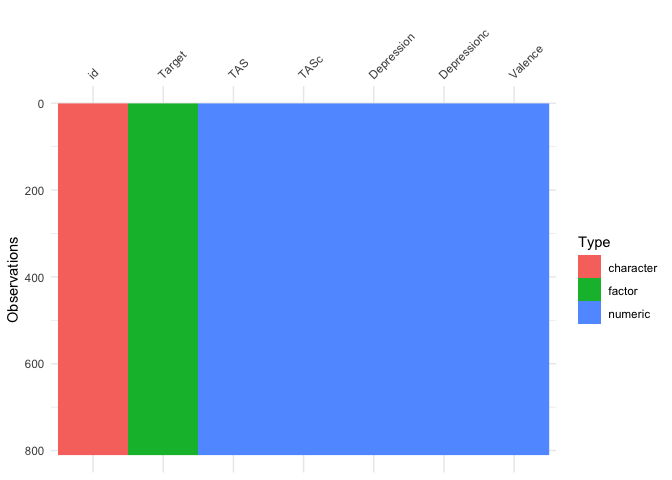
\includegraphics{ReviseResubmit_CleanedCode_files/figure-latex/valence long-1.pdf}

\hypertarget{arousal}{%
\subsection{Arousal}\label{arousal}}

\begin{Shaded}
\begin{Highlighting}[]
\NormalTok{LongA <-}\StringTok{ }\NormalTok{RRraw }\OperatorTok\StringTok{ }\KeywordTok{select}\NormalTok{(id,}
\NormalTok{                          TAS,}
\NormalTok{                          TASc,}
                          \KeywordTok{contains}\NormalTok{(}\StringTok{"Depression"}\NormalTok{),}
                          \KeywordTok{contains}\NormalTok{(}\StringTok{"Arousal"}\NormalTok{)) }\OperatorTok\StringTok{ }\KeywordTok{gather}\NormalTok{( }
                \DataTypeTok{key =} \StringTok{"Target"}\NormalTok{,}
                \DataTypeTok{value =} \StringTok{"Arousal"}\NormalTok{,}
\NormalTok{                TenderArousal, HappyArousal, AngryArousal, SadArousal, FearArousal, }
                \DataTypeTok{factor_key =} \OtherTok{TRUE}\NormalTok{) }

\NormalTok{LongA}\OperatorTok{$}\NormalTok{Target <-}\StringTok{  }\KeywordTok{recode}\NormalTok{(LongA}\OperatorTok{$}\NormalTok{Target, }
                 \DataTypeTok{TenderArousal =} \StringTok{"Tender"}\NormalTok{,}
                 \DataTypeTok{HappyArousal =} \StringTok{"Happy"}\NormalTok{,}
                 \DataTypeTok{AngryArousal =} \StringTok{"Angry"}\NormalTok{,}
                 \DataTypeTok{SadArousal =} \StringTok{"Sad"}\NormalTok{,}
                 \DataTypeTok{FearArousal =} \StringTok{"Fear"}\NormalTok{)}

\KeywordTok{levels}\NormalTok{(LongA}\OperatorTok{$}\NormalTok{Target)}
\end{Highlighting}
\end{Shaded}

\begin{verbatim}
## [1] "Tender" "Happy"  "Angry"  "Sad"    "Fear"
\end{verbatim}

\begin{Shaded}
\begin{Highlighting}[]
\NormalTok{visdat}\OperatorTok{::}\KeywordTok{vis_dat}\NormalTok{(LongA)}
\end{Highlighting}
\end{Shaded}

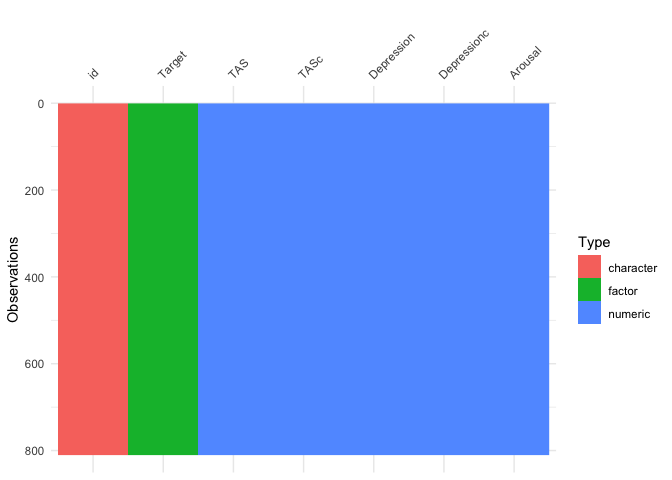
\includegraphics{ReviseResubmit_CleanedCode_files/figure-latex/arousal long-1.pdf}

\hypertarget{model-data}{%
\section{Model Data}\label{model-data}}

\hypertarget{valence-data}{%
\subsection{Valence Data}\label{valence-data}}

\begin{Shaded}
\begin{Highlighting}[]
\NormalTok{ValenceModelALX <-}\StringTok{ }\NormalTok{lme4}\OperatorTok{::}\KeywordTok{lmer}\NormalTok{(Valence}\OperatorTok{~}\NormalTok{TAS}\OperatorTok{*}\NormalTok{Target }\OperatorTok{+}\StringTok{ }\NormalTok{(}\DecValTok{1}\OperatorTok{|}\NormalTok{id), }\DataTypeTok{data =}\NormalTok{ LongV) }\CommentTok{# Hypothesised model }

\NormalTok{ValenceModelDepControl <-}\StringTok{ }\NormalTok{lme4}\OperatorTok{::}\KeywordTok{lmer}\NormalTok{(Valence}\OperatorTok{~}\NormalTok{Target}\OperatorTok{*}\NormalTok{TAS }\OperatorTok{+}\StringTok{ }\NormalTok{Depression }\OperatorTok{+}\StringTok{ }\NormalTok{(}\DecValTok{1}\OperatorTok{|}\NormalTok{id), }\DataTypeTok{data =}\NormalTok{ LongV) }\CommentTok{# Add depression}

\NormalTok{ValenceModelDepInt <-}\StringTok{ }\NormalTok{lme4}\OperatorTok{::}\KeywordTok{lmer}\NormalTok{(Valence}\OperatorTok{~}\NormalTok{Target}\OperatorTok{*}\NormalTok{TAS}\OperatorTok{*}\NormalTok{Depression }\OperatorTok{+}\StringTok{ }\NormalTok{(}\DecValTok{1}\OperatorTok{|}\NormalTok{id), }\DataTypeTok{data =}\NormalTok{ LongV) }\CommentTok{# 3 way interaction }

\KeywordTok{anova}\NormalTok{(ValenceModelALX, ValenceModelDepControl, ValenceModelDepInt) }\CommentTok{# compared models - all }
\end{Highlighting}
\end{Shaded}

\begin{verbatim}
## refitting model(s) with ML (instead of REML)
\end{verbatim}

\begin{verbatim}
## Data: LongV
## Models:
## ValenceModelALX: Valence ~ TAS * Target + (1 | id)
## ValenceModelDepControl: Valence ~ Target * TAS + Depression + (1 | id)
## ValenceModelDepInt: Valence ~ Target * TAS * Depression + (1 | id)
##                        Df    AIC    BIC  logLik deviance   Chisq Chi Df
## ValenceModelALX        12 2406.3 2462.7 -1191.2   2382.3               
## ValenceModelDepControl 13 2408.3 2469.4 -1191.2   2382.3  0.0274      1
## ValenceModelDepInt     22 2415.6 2518.9 -1185.8   2371.6 10.7394      9
##                        Pr(>Chisq)
## ValenceModelALX                  
## ValenceModelDepControl     0.8686
## ValenceModelDepInt         0.2940
\end{verbatim}

\begin{Shaded}
\begin{Highlighting}[]
\KeywordTok{anova}\NormalTok{(ValenceModelALX, ValenceModelDepInt) }\CommentTok{# compare hypothesised and 3 way interaction}
\end{Highlighting}
\end{Shaded}

\begin{verbatim}
## refitting model(s) with ML (instead of REML)
\end{verbatim}

\begin{verbatim}
## Data: LongV
## Models:
## ValenceModelALX: Valence ~ TAS * Target + (1 | id)
## ValenceModelDepInt: Valence ~ Target * TAS * Depression + (1 | id)
##                    Df    AIC    BIC  logLik deviance  Chisq Chi Df
## ValenceModelALX    12 2406.3 2462.7 -1191.2   2382.3              
## ValenceModelDepInt 22 2415.6 2518.9 -1185.8   2371.6 10.767     10
##                    Pr(>Chisq)
## ValenceModelALX              
## ValenceModelDepInt      0.376
\end{verbatim}

\begin{Shaded}
\begin{Highlighting}[]
\NormalTok{sjPlot}\OperatorTok{::}\KeywordTok{tab_model}\NormalTok{(ValenceModelALX, ValenceModelDepInt) }
\end{Highlighting}
\end{Shaded}

\begin{verbatim}
## Computing p-values via Wald-statistics approximation (treating t as Wald z).
\end{verbatim}

\begin{verbatim}
## Computing p-values via Wald-statistics approximation (treating t as Wald z).
\end{verbatim}

~

Valence

Valence

Predictors

Estimates

CI

p

Estimates

CI

p

(Intercept)

0.86

0.09~--~1.62

0.029

0.33

-0.78~--~1.43

0.561

TAS

-0.00

-0.02~--~0.01

0.776

0.01

-0.01~--~0.03

0.478

Happy

1.87

0.83~--~2.91

\textless0.001

2.26

0.77~--~3.75

0.003

Angry

-2.80

-3.84~--~-1.76

\textless0.001

-1.54

-3.04~--~-0.05

0.042

Sad

-3.26

-4.30~--~-2.22

\textless0.001

-2.60

-4.09~--~-1.11

0.001

Fear

-3.38

-4.42~--~-2.34

\textless0.001

-2.60

-4.09~--~-1.11

0.001

TAS:TargetHappy

-0.01

-0.03~--~0.01

0.441

TAS:TargetAngry

0.02

0.00~--~0.04

0.044

TAS:TargetSad

0.03

0.01~--~0.05

0.003

TAS:TargetFear

0.02

0.00~--~0.04

0.025

Depression

0.12

-0.05~--~0.29

0.173

TargetHappy:TAS

-0.01

-0.04~--~0.01

0.314

TargetAngry:TAS

-0.00

-0.03~--~0.03

0.878

TargetSad:TAS

0.01

-0.01~--~0.04

0.332

TargetFear:TAS

0.01

-0.02~--~0.04

0.577

TargetHappy:Depression

-0.08

-0.31~--~0.15

0.498

TargetAngry:Depression

-0.32

-0.55~--~-0.09

0.006

TargetSad:Depression

-0.10

-0.33~--~0.13

0.382

TargetFear:Depression

-0.21

-0.43~--~0.02

0.077

TAS:Depression

-0.00

-0.00~--~0.00

0.163

TargetHappy:TAS:Depression

0.00

-0.00~--~0.01

0.470

TargetAngry:TAS:Depression

0.01

0.00~--~0.01

0.008

TargetSad:TAS:Depression

0.00

-0.00~--~0.01

0.294

TargetFear:TAS:Depression

0.00

-0.00~--~0.01

0.090

Random Effects

σ2

1.04

1.04

τ00

0.10 id

0.10 id

ICC

0.08 id

0.09 id

Observations

810

810

Marginal R2 / Conditional R2

0.631 / 0.662

0.633 / 0.665

\begin{Shaded}
\begin{Highlighting}[]
\NormalTok{sjPlot}\OperatorTok{::}\KeywordTok{tab_model}\NormalTok{(ValenceModelALX)}
\end{Highlighting}
\end{Shaded}

\begin{verbatim}
## Computing p-values via Wald-statistics approximation (treating t as Wald z).
\end{verbatim}

~

Valence

Predictors

Estimates

CI

p

(Intercept)

0.86

0.09~--~1.62

0.029

TAS

-0.00

-0.02~--~0.01

0.776

Happy

1.87

0.83~--~2.91

\textless0.001

Angry

-2.80

-3.84~--~-1.76

\textless0.001

Sad

-3.26

-4.30~--~-2.22

\textless0.001

Fear

-3.38

-4.42~--~-2.34

\textless0.001

TAS:TargetHappy

-0.01

-0.03~--~0.01

0.441

TAS:TargetAngry

0.02

0.00~--~0.04

0.044

TAS:TargetSad

0.03

0.01~--~0.05

0.003

TAS:TargetFear

0.02

0.00~--~0.04

0.025

Random Effects

σ2

1.04

τ00 id

0.10

ICC id

0.08

Observations

810

Marginal R2 / Conditional R2

0.631 / 0.662

\begin{Shaded}
\begin{Highlighting}[]
\NormalTok{interactions}\OperatorTok{::}\KeywordTok{sim_slopes}\NormalTok{(}\DataTypeTok{model =}\NormalTok{ ValenceModelALX, }\DataTypeTok{pred =}\NormalTok{ TAS, }\DataTypeTok{modx =}\NormalTok{ Target)}
\end{Highlighting}
\end{Shaded}

\begin{verbatim}
## Warning: Johnson-Neyman intervals are not available for factor moderators.
\end{verbatim}

\begin{verbatim}
## SIMPLE SLOPES ANALYSIS 
## 
## Slope of TAS when Target = Fear: 
## 
##   Est.   S.E.   t val.      p
## ------ ------ -------- ------
##   0.02   0.01     2.75   0.01
## 
## Slope of TAS when Target = Sad: 
## 
##   Est.   S.E.   t val.      p
## ------ ------ -------- ------
##   0.03   0.01     3.76   0.00
## 
## Slope of TAS when Target = Angry: 
## 
##   Est.   S.E.   t val.      p
## ------ ------ -------- ------
##   0.02   0.01     2.44   0.01
## 
## Slope of TAS when Target = Happy: 
## 
##    Est.   S.E.   t val.      p
## ------- ------ -------- ------
##   -0.01   0.01    -1.33   0.19
## 
## Slope of TAS when Target = Tender: 
## 
##    Est.   S.E.   t val.      p
## ------- ------ -------- ------
##   -0.00   0.01    -0.28   0.78
\end{verbatim}

\begin{Shaded}
\begin{Highlighting}[]
\NormalTok{sjPlot}\OperatorTok{::}\KeywordTok{plot_model}\NormalTok{(ValenceModelALX, }
                   \DataTypeTok{type =} \StringTok{"int"}\NormalTok{,}
                   \DataTypeTok{title =} \StringTok{""}\NormalTok{,}
                   \DataTypeTok{axis.title =} \KeywordTok{c}\NormalTok{(}\StringTok{"Alexithymia Score"}\NormalTok{, }\StringTok{"Rated Valence"}\NormalTok{),}
                   \DataTypeTok{legend.title =} \StringTok{"Target Emotion"}\NormalTok{) }\OperatorTok{+}\StringTok{ }
\StringTok{  }\NormalTok{ggplot2}\OperatorTok{::}\KeywordTok{theme_classic}\NormalTok{() }\OperatorTok{+}
\StringTok{  }\NormalTok{ggplot2}\OperatorTok{::}\KeywordTok{scale_y_continuous}\NormalTok{(}\DataTypeTok{name =} \StringTok{"Rated Valence"}\NormalTok{, }\DataTypeTok{breaks =} \KeywordTok{c}\NormalTok{(}\OperatorTok{-}\DecValTok{3}\NormalTok{, }\DecValTok{-2}\NormalTok{, }\DecValTok{-1}\NormalTok{, }\DecValTok{0}\NormalTok{, }\DecValTok{1}\NormalTok{, }\DecValTok{2}\NormalTok{, }\DecValTok{3}\NormalTok{), }\DataTypeTok{limits =} \KeywordTok{c}\NormalTok{(}\OperatorTok{-}\DecValTok{3}\NormalTok{,}\DecValTok{3}\NormalTok{)) }\OperatorTok{+}
\StringTok{  }\NormalTok{ggplot2}\OperatorTok{::}\KeywordTok{geom_hline}\NormalTok{(}\DataTypeTok{yintercept =} \DecValTok{0}\NormalTok{, }\DataTypeTok{linetype =} \StringTok{"dotted"}\NormalTok{) }
\end{Highlighting}
\end{Shaded}

\begin{verbatim}
## Scale for 'y' is already present. Adding another scale for 'y', which
## will replace the existing scale.
\end{verbatim}

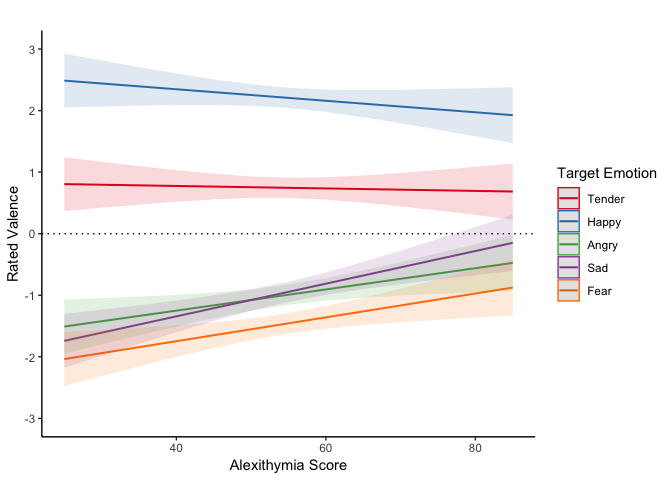
\includegraphics{ReviseResubmit_CleanedCode_files/figure-latex/valence model-1.pdf}

\hypertarget{arousal-data}{%
\subsection{Arousal Data}\label{arousal-data}}

\begin{Shaded}
\begin{Highlighting}[]
\NormalTok{ArousalModelALX <-}\StringTok{ }\NormalTok{lme4}\OperatorTok{::}\KeywordTok{lmer}\NormalTok{(Arousal}\OperatorTok{~}\NormalTok{TAS}\OperatorTok{*}\NormalTok{Target }\OperatorTok{+}\StringTok{ }\NormalTok{(}\DecValTok{1}\OperatorTok{|}\NormalTok{id), }\DataTypeTok{data =}\NormalTok{ LongA) }\CommentTok{# Hypothesised model }

\NormalTok{ArousalModelDepControl <-}\StringTok{ }\NormalTok{lme4}\OperatorTok{::}\KeywordTok{lmer}\NormalTok{(Arousal}\OperatorTok{~}\NormalTok{Target}\OperatorTok{*}\NormalTok{TAS }\OperatorTok{+}\StringTok{ }\NormalTok{Depression }\OperatorTok{+}\StringTok{ }\NormalTok{(}\DecValTok{1}\OperatorTok{|}\NormalTok{id), }\DataTypeTok{data =}\NormalTok{ LongA) }\CommentTok{# Add depression}

\NormalTok{ArousalModelDepInt <-}\StringTok{ }\NormalTok{lme4}\OperatorTok{::}\KeywordTok{lmer}\NormalTok{(Arousal}\OperatorTok{~}\NormalTok{Target}\OperatorTok{*}\NormalTok{TAS}\OperatorTok{*}\NormalTok{Depression }\OperatorTok{+}\StringTok{ }\NormalTok{(}\DecValTok{1}\OperatorTok{|}\NormalTok{id), }\DataTypeTok{data =}\NormalTok{ LongA) }\CommentTok{# 3 way interaction }

\KeywordTok{anova}\NormalTok{(ArousalModelALX, ArousalModelDepControl, ArousalModelDepInt) }\CommentTok{# compared models - all }
\end{Highlighting}
\end{Shaded}

\begin{verbatim}
## refitting model(s) with ML (instead of REML)
\end{verbatim}

\begin{verbatim}
## Data: LongA
## Models:
## ArousalModelALX: Arousal ~ TAS * Target + (1 | id)
## ArousalModelDepControl: Arousal ~ Target * TAS + Depression + (1 | id)
## ArousalModelDepInt: Arousal ~ Target * TAS * Depression + (1 | id)
##                        Df    AIC    BIC  logLik deviance  Chisq Chi Df
## ArousalModelALX        12 2509.0 2565.4 -1242.5   2485.0              
## ArousalModelDepControl 13 2510.7 2571.7 -1242.3   2484.7 0.3532      1
## ArousalModelDepInt     22 2522.3 2625.7 -1239.2   2478.3 6.3459      9
##                        Pr(>Chisq)
## ArousalModelALX                  
## ArousalModelDepControl     0.5523
## ArousalModelDepInt         0.7049
\end{verbatim}

\begin{Shaded}
\begin{Highlighting}[]
\KeywordTok{anova}\NormalTok{(ArousalModelALX, ArousalModelDepInt) }\CommentTok{# compare hypothesised and 3 way interaction}
\end{Highlighting}
\end{Shaded}

\begin{verbatim}
## refitting model(s) with ML (instead of REML)
\end{verbatim}

\begin{verbatim}
## Data: LongA
## Models:
## ArousalModelALX: Arousal ~ TAS * Target + (1 | id)
## ArousalModelDepInt: Arousal ~ Target * TAS * Depression + (1 | id)
##                    Df    AIC    BIC  logLik deviance  Chisq Chi Df
## ArousalModelALX    12 2509.0 2565.4 -1242.5   2485.0              
## ArousalModelDepInt 22 2522.3 2625.7 -1239.2   2478.3 6.6991     10
##                    Pr(>Chisq)
## ArousalModelALX              
## ArousalModelDepInt     0.7535
\end{verbatim}

\begin{Shaded}
\begin{Highlighting}[]
\NormalTok{sjPlot}\OperatorTok{::}\KeywordTok{tab_model}\NormalTok{(ArousalModelALX, ArousalModelDepInt) }
\end{Highlighting}
\end{Shaded}

\begin{verbatim}
## Computing p-values via Wald-statistics approximation (treating t as Wald z).
\end{verbatim}

\begin{verbatim}
## Computing p-values via Wald-statistics approximation (treating t as Wald z).
\end{verbatim}

~

Arousal

Arousal

Predictors

Estimates

CI

p

Estimates

CI

p

(Intercept)

0.86

0.03~--~1.68

0.041

0.33

-0.85~--~1.51

0.587

TAS

-0.00

-0.02~--~0.01

0.790

0.01

-0.02~--~0.03

0.507

Happy

1.46

0.36~--~2.56

0.009

1.89

0.31~--~3.48

0.019

Angry

1.93

0.83~--~3.03

0.001

1.84

0.26~--~3.42

0.023

Sad

-3.71

-4.81~--~-2.61

\textless0.001

-2.76

-4.35~--~-1.18

0.001

Fear

0.76

-0.34~--~1.86

0.178

0.95

-0.64~--~2.53

0.242

TAS:TargetHappy

-0.00

-0.02~--~0.02

0.900

TAS:TargetAngry

-0.03

-0.05~--~-0.01

0.006

TAS:TargetSad

0.03

0.01~--~0.05

0.002

TAS:TargetFear

-0.02

-0.03~--~0.00

0.136

Depression

0.12

-0.06~--~0.30

0.202

TargetHappy:TAS

-0.01

-0.04~--~0.02

0.598

TargetAngry:TAS

-0.02

-0.05~--~0.01

0.129

TargetSad:TAS

0.02

-0.02~--~0.05

0.340

TargetFear:TAS

-0.02

-0.05~--~0.01

0.231

TargetHappy:Depression

-0.12

-0.37~--~0.12

0.323

TargetAngry:Depression

-0.03

-0.28~--~0.21

0.789

TargetSad:Depression

-0.23

-0.47~--~0.02

0.068

TargetFear:Depression

-0.03

-0.28~--~0.21

0.789

TAS:Depression

-0.00

-0.00~--~0.00

0.192

TargetHappy:TAS:Depression

0.00

-0.00~--~0.01

0.353

TargetAngry:TAS:Depression

0.00

-0.00~--~0.00

0.919

TargetSad:TAS:Depression

0.00

-0.00~--~0.01

0.070

TargetFear:TAS:Depression

0.00

-0.00~--~0.00

0.762

Random Effects

σ2

1.17

1.17

τ00

0.13 id

0.13 id

ICC

0.10 id

0.10 id

Observations

810

810

Marginal R2 / Conditional R2

0.492 / 0.543

0.493 / 0.545

\begin{Shaded}
\begin{Highlighting}[]
\NormalTok{sjPlot}\OperatorTok{::}\KeywordTok{tab_model}\NormalTok{(ArousalModelALX)}
\end{Highlighting}
\end{Shaded}

\begin{verbatim}
## Computing p-values via Wald-statistics approximation (treating t as Wald z).
\end{verbatim}

~

Arousal

Predictors

Estimates

CI

p

(Intercept)

0.86

0.03~--~1.68

0.041

TAS

-0.00

-0.02~--~0.01

0.790

Happy

1.46

0.36~--~2.56

0.009

Angry

1.93

0.83~--~3.03

0.001

Sad

-3.71

-4.81~--~-2.61

\textless0.001

Fear

0.76

-0.34~--~1.86

0.178

TAS:TargetHappy

-0.00

-0.02~--~0.02

0.900

TAS:TargetAngry

-0.03

-0.05~--~-0.01

0.006

TAS:TargetSad

0.03

0.01~--~0.05

0.002

TAS:TargetFear

-0.02

-0.03~--~0.00

0.136

Random Effects

σ2

1.17

τ00 id

0.13

ICC id

0.10

Observations

810

Marginal R2 / Conditional R2

0.492 / 0.543

\begin{Shaded}
\begin{Highlighting}[]
\NormalTok{interactions}\OperatorTok{::}\KeywordTok{sim_slopes}\NormalTok{(}\DataTypeTok{model =}\NormalTok{ ArousalModelALX, }\DataTypeTok{pred =}\NormalTok{ TAS, }\DataTypeTok{modx =}\NormalTok{ Target)}
\end{Highlighting}
\end{Shaded}

\begin{verbatim}
## Warning: Johnson-Neyman intervals are not available for factor moderators.
\end{verbatim}

\begin{verbatim}
## SIMPLE SLOPES ANALYSIS 
## 
## Slope of TAS when Target = Fear: 
## 
##    Est.   S.E.   t val.      p
## ------- ------ -------- ------
##   -0.02   0.01    -2.27   0.02
## 
## Slope of TAS when Target = Sad: 
## 
##   Est.   S.E.   t val.      p
## ------ ------ -------- ------
##   0.03   0.01     3.97   0.00
## 
## Slope of TAS when Target = Angry: 
## 
##    Est.   S.E.   t val.      p
## ------- ------ -------- ------
##   -0.03   0.01    -3.96   0.00
## 
## Slope of TAS when Target = Happy: 
## 
##    Est.   S.E.   t val.      p
## ------- ------ -------- ------
##   -0.00   0.01    -0.43   0.66
## 
## Slope of TAS when Target = Tender: 
## 
##    Est.   S.E.   t val.      p
## ------- ------ -------- ------
##   -0.00   0.01    -0.27   0.79
\end{verbatim}

\begin{Shaded}
\begin{Highlighting}[]
\NormalTok{sjPlot}\OperatorTok{::}\KeywordTok{plot_model}\NormalTok{(ArousalModelALX, }
                   \DataTypeTok{type =} \StringTok{"int"}\NormalTok{,}
                   \DataTypeTok{title =} \StringTok{""}\NormalTok{,}
                   \DataTypeTok{axis.title =} \KeywordTok{c}\NormalTok{(}\StringTok{"Alexithymia Score"}\NormalTok{, }\StringTok{"Rated Arousal"}\NormalTok{),}
                   \DataTypeTok{legend.title =} \StringTok{"Target Emotion"}\NormalTok{) }\OperatorTok{+}\StringTok{ }
\NormalTok{ggplot2}\OperatorTok{::}\KeywordTok{scale_y_continuous}\NormalTok{(}\DataTypeTok{name =} \StringTok{"Rated Arousal"}\NormalTok{, }\DataTypeTok{breaks =} \KeywordTok{c}\NormalTok{(}\OperatorTok{-}\DecValTok{3}\NormalTok{, }\DecValTok{-2}\NormalTok{, }\DecValTok{-1}\NormalTok{, }\DecValTok{0}\NormalTok{, }\DecValTok{1}\NormalTok{, }\DecValTok{2}\NormalTok{, }\DecValTok{3}\NormalTok{), }\DataTypeTok{limits =} \KeywordTok{c}\NormalTok{(}\OperatorTok{-}\DecValTok{3}\NormalTok{,}\DecValTok{3}\NormalTok{)) }\OperatorTok{+}
\StringTok{  }\NormalTok{ggplot2}\OperatorTok{::}\KeywordTok{theme_classic}\NormalTok{() }\OperatorTok{+}
\StringTok{  }\NormalTok{ggplot2}\OperatorTok{::}\KeywordTok{geom_hline}\NormalTok{(}\DataTypeTok{yintercept =} \DecValTok{0}\NormalTok{, }\DataTypeTok{linetype =} \StringTok{"dotted"}\NormalTok{)     }
\end{Highlighting}
\end{Shaded}

\begin{verbatim}
## Scale for 'y' is already present. Adding another scale for 'y', which
## will replace the existing scale.
\end{verbatim}

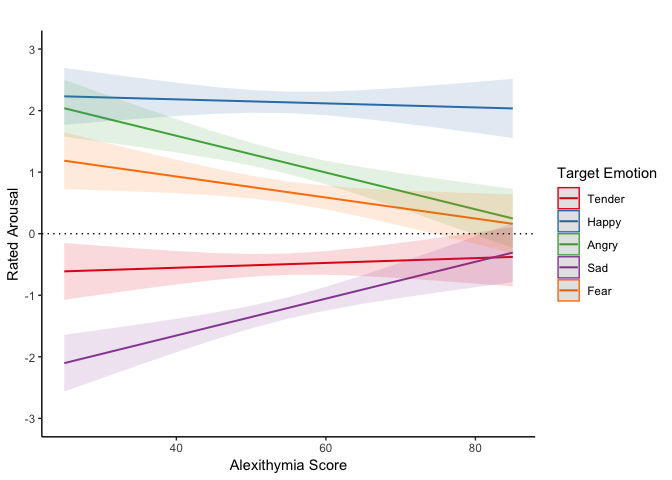
\includegraphics{ReviseResubmit_CleanedCode_files/figure-latex/arousal model-1.pdf}


\end{document}
